% Intended LaTeX compiler: pdflatex
\documentclass[10pt,a4paper,UTF8]{article}
\usepackage{zclorg}
\author{张朝龙}
\date{}
\title{练习:本证空间}
\hypersetup{
 pdfauthor={张朝龙},
 pdftitle={练习:本证空间},
 pdfkeywords={},
 pdfsubject={},
 pdfcreator={Emacs 25.0.50.1 (Org mode 9.0.6)},
 pdflang={English}}
\begin{document}

\maketitle
\tableofcontents
\titlepic{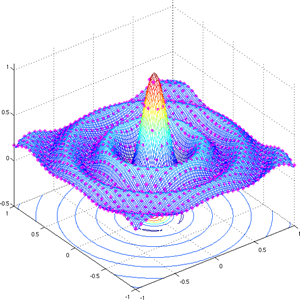
\includegraphics[scale=0.25]{../../img/sinc.PNG}}


\section{5.C.1}
\label{sec:orge84f6c2}


\begin{problem}
设\(T\in \mathcal{L}(V)\)可对角化,证明\(V = \mathrm{null}(T) \oplus \mathrm{range}(T)\)
\end{problem}

\begin{answer}
对于\(T\in \mathcal{L}(V)\),假设\(\lambda_{1},\ldots ,\lambda_{m}\)是\(T\)的互异的本征值,则:
\begin{enumerate}
\item \(T\)可对角化。
\item \(V\)有由\(T\)的本证向量构成的基;
\item \(V\)有在\(T\)下不变的一维子空间\(U_{1},\ldots ,U_{n}\)使得\(V= U_{1}\oplus + \ldots + U_{n}\)
\item \(V = E(\lambda_{1},T) \oplus \ldots \oplus E(\lambda_{m},T)\)
\item \(\dim V = \dim E(\lambda_{1},T) + \ldots + \dim E(\lambda_{m},T)\)
\end{enumerate}

对于这个题目我们可以把特征向量分为两类,一类特征向量是特征值\(0\)对应的特征向量,一类特征向量是非零特征值对应的特征向量。基本证明思路已经比较清晰了。接下类给出详细的证明过程。

如果\(T\)是可逆的,那么\(\mathrm{null}T = \{0\}\),\(\mathrm{range}T = V\),此时\(T\)是单射也是满射,显然有\(V = \mathrm{null}T \oplus \mathrm{range}T\),证明完毕。

如果\(T\)不是可逆的,假设\(0,\lambda_{1},\ldots ,\lambda_{m}\)是\(T\)的特征值。所以有:
\begin{equation}
\label{eq:1}
V = E(0,T) \oplus  E(\lambda_{1},T) \oplus \ldots \oplus E(\lambda_{m},T)
\end{equation}
利用定义我们有\(E(0,T) = \mathrm{null}T\)。另外
\[T(\frac{1}{\lambda_{j}}v_{j}) = v_{j}\]
所以\(E(\lambda_{j},T)\subset \mathrm{range}T\),因此
\[E(\lambda_{1},T)\oplus \ldots \oplus E(\lambda_{m},T) \subset \mathrm{range}T\]
另一方面,对于任何\(v\in V\),可以写作:
\[v= v_{0} + v_{1} + \ldots +v_{m}\]
其中\(v_{0}\in E(0,T),v_{j}\in E(\lambda_{j},T)\),因此:
\[T(v) = T(v_{0}+ v_{1} + \ldots v_{m}) = \lambda_{1}v_{1} + \ldots  +\lambda_{m}v_{m} \in E(\lambda_{1},T) \oplus \ldots \oplus E(\lambda_{m},T)\]
因此有:
\[\mathrm{range}T = E(\lambda_{1},T) \oplus \ldots \oplus E(\lambda_{m},T) \]
因此\(V = \mathrm{null}T \oplus \mathrm{range}T\)

对于这个题目虽然我想到了最主要的思路。但是在执行细节上我没有按照定理来做,子集创造了很多结论。
\end{answer}
\section{5.C.3}
\label{sec:orge564890}


\begin{problem}
设\(V\)是有限维的且\(T\in \mathcal{L}(V)\),证明下列命题等价
\begin{enumerate}
\item \(V = \mathrm{null}T \oplus \mathrm{range}T\)
\item \(V = \mathrm{null}T + \mathrm{range}T\)
\item \(\mathrm{null}T \cap \mathrm{range}T = \{0\}\)
\end{enumerate}
\end{problem}

\begin{answer}
证明从1到2是显然的。我们证明从2到3.

因为
\[V = \mathrm{null}T + \mathrm{range}T\]
所以
\[\dim V = \dim \mathrm{null}T + \dim \mathrm{range}T - \dim (\mathrm{null}T \cap + \mathrm{range}T)\]
根据线性映射基本定理:
\[\dim V = \dim \mathrm{null}T + \dim \mathrm{range}T\]
所以我们有:
\[0 = \dim (\mathrm{null}T \cap + \mathrm{range}T)\]
因此
\[ \{0\} = \mathrm{null}T \cap + \mathrm{range}T\]

证明从3到1 :
因为
\[\mathrm{null}T \cap \mathrm{range}T = \{0\}\]
所以
\[\dim V = \dim \mathrm{null}T + \dim \mathrm{range}T\]
进而有:
\[\dim V = \dim (\mathrm{null}T + \mathrm{range}T)\]
因此\(\mathrm{null}T + \mathrm{range}T = V\),又因为\(\mathrm{null}T \cap \mathrm{range}T = \{0\}\),所以\(\mathrm{null}T \oplus \mathrm{range}T = V\)
\end{answer}

\section{5.C.5}
\label{sec:org6d8d972}


\begin{problem}
设\(V\)是有限维的复向量空间且\(T\in \mathcal{L}(V)\),证明:\(T\)可对角化当且仅当对每个\(\lambda \in \mathbf{C}\)有\(V = \mathrm{null}(T-\lambda I) \oplus \mathrm{range}(T-\lambda I)\)
\end{problem}

\begin{answer}
首先假设\(T\)可以对角化,则\(T-\lambda I\)也可以对角化,因此利用5.C.1的结论有:
\begin{equation}
\label{eq:2}
V= \mathrm{null}(T-\lambda I) \oplus \mathrm{range}(T-\lambda I)
\end{equation}

然后我们证明另外一个方向,因为\(V\)是有限维的,所以\(T\)有有限个特征值。假设\(\lambda_{1},\ldots ,\lambda_{m}\)是\(T\)的不同的特征值,所以:
\begin{equation}
\label{eq:3}
T = \mathrm{null}(T-\lambda_{1} I) \oplus \mathrm{range}(T-\lambda_{1} I)
\end{equation}
且有:\(\mathrm{null}(T-\lambda_{2}I) \subset \mathrm{range}(T-\lambda_{1} I)\),我们有:
\begin{equation}
\label{eq:4}
\mathrm{range}(T-\lambda_{1}I) = \mathrm{null}(T-\lambda_{2} I)\oplus \mathrm{range}(T-\lambda_{1}I)\cap \mathrm{range}(T-\lambda_{2}I)
\end{equation}
同样的我们有:
\begin{equation}
\label{eq:5}
\mathrm{null}(T-\lambda_{3}I)\subset \mathrm{range}(T-\lambda_{1}I)\cap \mathrm{range}(T-\lambda_{2}I)
\end{equation}
进而有:
\begin{equation}
\label{eq:6}
V = null(T-\lambda_{1}I)\oplus \ldots \oplus \mathrm{null}(T-\lambda_{m}I) \oplus (\mathrm{range}(T-\lambda_{1}I) \cap \ldots \cap \mathrm{range}(T-\lambda_{m}I))
\end{equation}
如果:\(\mathrm{range}(T-\lambda_{1}I) \cap \ldots \cap \mathrm{range}(T-\lambda_{m}I) = \{0\}\),那么:
\begin{equation}
\label{eq:7}
V = null(T-\lambda_{1}I)\oplus \ldots \oplus \mathrm{null}(T-\lambda_{m}I)
\end{equation}
所以\(T\)是可对角化的。
如果\(\mathrm{range}(T-\lambda_{1}I) \cap \ldots \cap \mathrm{range}(T-\lambda_{m}I) \neq \{0\}\),因为\((T-\lambda_{i}I)T = T(T-\lambda_{i}I)\),所以我们有\(\mathrm{range}(T-\lambda_{i}I)\)在\(T\)下是不变的。\(.......\)接下来证明不下去了
\end{answer}
\section{5.C.6}
\label{sec:org301aad0}


\begin{problem}
设\(V\)是有限维的,\(T\in \mathcal{L}(V)\)有\(\dim V\)个互异的本征值,\(S\in \mathcal{L}(V)\)与\(T\)有相同的本证向量(未必相应于同一本征值),证明\(TS = ST\)
\end{problem}

\begin{answer}
因为\(T\)有\(\dim V\)个互异的本证值,则我们可以找出\(V\)的一个基\(v_{1},\ldots ,v_{\dim V}\)使其是\(T\)的对应于\(\dim V\)个互异的本征值的本证向量。

因为\(S\in \mathcal{L}(V)\)和\(T\)有相同的本证向量,那么存在\(\lambda_{1},\ldots ,\lambda_{\dim V}\)和\(\theta_{1},\ldots ,\theta_{\dim V}\)使得:
\begin{equation}
\label{eq:8}
Tv_{i} = \lambda_{i}v_{i},\quad Sv_{i} = \theta_{i}v_{i}
\end{equation}
所以我们有:
\begin{equation}
\label{eq:9}
STv_{i} = S(\lambda_{i}v_{i}) = \lambda_{i}Sv_{i} = \lambda_{i}\theta_{i} v_{i},i=1,\ldots ,\dim V
\end{equation}
\begin{equation}
\label{eq:10}
TSv_{i} = T(\theta_{i}v_{i}) = \theta_{i}Tv_{i} = \theta_{i}\lambda_{i}v_{i} ,i = 1,\ldots ,\dim V
\end{equation}
所以\(STv_{i} = TSv_{i},i=1,\ldots ,\dim V\),因为\(v_{1},\ldots ,\dim V\)是\(V\)的一个基。所以\(ST=TS\)
\end{answer}
\section{5.C.8}
\label{sec:org53d4aed}


\begin{problem}
设\(T\in \mathbf{F}^{5}\)且\(\dim E(8,T) = 4\)。证明\(T-2\lambda\)或者\(T-6\lambda\)是可逆的。
\end{problem}

\begin{answer}
反证法。假设\(T-2\lambda\)和\(T-6\lambda\)是不可逆的,这意味着\(2\)和\(6\)是\(T\)的特征值,因此\(\dim E(2,T)\geq 1\),且\(\dim E(6,T)\geq 1\)所以有:
\begin{equation}
\label{eq:11}
4 + 1 + 1 \leq \dim E(8,T) + \dim E(2,T) + \dim E(6,T) \leq \dim V = 5
\end{equation}
矛盾。所以假设错误,所以有\(T-2\lambda\)或者\(T-6\lambda\)是可逆的。
\end{answer}
\section{5.C.9}
\label{sec:org379c3d8}


\begin{problem}
设\(T\in \mathcal{L}(V)\)是可逆的。证明对每个非零的\(\lambda\)均有\(E(\lambda,T) = E(\frac{1}{\lambda},T^{-1})\)
\end{problem}

\begin{answer}
\(\forall \lambda \in \mathbf{F},\lambda\neq 0\),令\(v\in E(\lambda,T)\),则\(Tv = \lambda v\),注意对于\(\lambda,\lambda\neq 0\),有\(Tv = \lambda v\)。由于\(T\)可逆,所以\(\frac{1}{\lambda}v = T^{-1}v\),因此\(v\in E( \frac{1}{\lambda},T^{-1})\),因此\(E(\lambda,T)\subset E(\frac{1}{\lambda},T^{-1})\).

同理,我们可以证明\(E(\frac{1}{\lambda},T^{-1}) \subset E(\lambda,T)\)。因此\(E(\lambda,T) = E(\frac{1}{\lambda},T^{-1})\).
\end{answer}
\section{5.C.12}
\label{sec:org4ebf389}


\begin{problem}
设\(R,T\in \mathcal{L}( \mathbf{F}^{3} )\),本征值均为\(2,6,7\),证明存在可逆算子\(S\in \mathcal{L}( \mathbf{F}^{3} )\)使得\(R = S^{-1}TS\)
\end{problem}

\begin{answer}
因为对于\(\mathcal{L}(\mathbf{F}^{3})\)中的线性算子\(T,R\)有本征值\(2,6,7\),则说明\(T,R\)都是可对角化的。因此存在\(T\)的基\(e_{1},e_{2},e_{3}\)和\(R\)的基\(\xi_{1},\xi_{2},\xi_{3}\)使得:
\begin{eqnarray}
\label{eq:12}
& &Te_{1} = 2e_{1},Te_{2} = 6e_{2}, Te_{3} = 7e_{3} \\
& &R\xi_{1} = 2\xi_{1},R\xi_{2} = 6\xi_{2}, R\xi_{3} = 7\xi_{3}
\end{eqnarray}
定义\(S\in \mathcal{L}(\mathbf{F}^{3})\):对$\backslash$
\begin{equation}
\label{eq:13}
S\xi_{i} = e_{i},i = 1,2,3
\end{equation}
所以\(\xi_{i} = S^{-1}e_{i},i=1,2,3\)。所以:
\begin{equation}
\label{eq:14}
S^{-1}TS\xi_{1} = S^{-1}Te_{1} =  S^{-1} 2 e_{1} = 2 \xi_{1} = R\xi_{1}
\end{equation}
类似的,我们有\(S^{-1}TS \xi_{2} = R \xi_{2},S^{-1}TS\xi_{3} = R \xi_{3}\)。因为\(S^{-1}TS\)和\(S\)在基上的作用是相同的,所以\(S^{-1}TS = R\)
\end{answer}
\section{5.C.13}
\label{sec:orgf01880d}


\begin{problem}
求\(R,T\in \mathcal{L}(\mathbf{F}^{4})\)使得\(R\)和\(T\)均有本征值\(2,6,7\),均没有其他本征值,且不存在可逆算子\(S\in \mathcal{L}(\mathbf{F}^{4})\)使得\(R=S^{-1}TS\)
\end{problem}

\begin{answer}
令\(e_{1},\ldots ,e_{4}\)是\(\mathbf{F}^{4}\)的一个基,定义\(R,T\in \mathcal{L}(\mathbf{F}^{4})\):
\begin{equation}
\label{eq:15}
Re_{1} = 2e_{1},Re_{2} = 2e_{2},Re_{3} = 6e_{3},Re_{4} =7e_{4}
\end{equation}
\begin{equation}
\label{eq:16}
Te_{1} = 2e_{1}, Te_{2} = 2e_{2} + e_{1}, Te_{3} = 6e_{3},Te_{4} = 7e_{4}
\end{equation}
那么\(R\)是可对角化的,\(T\)不是可对角化的。

如果存在可逆映射\(S\in \mathcal{L}(\mathbf{F}^{4})\),满足\(R= S^{-1}TS\),\(SRS^{-1} = T\),那么\(Se_{1},\ldots ,Se_{4}\)是\(\mathbf{F}^{4}\)的一个基。进而:
\begin{equation}
\label{eq:17}
T(Se_{1}) = SRS^{-1}(Se_{1}) = SRe_{1} = S(2e_{1}) = 2Se_{1}
\end{equation}
同样:\(T(Se_{2}) = 2Se_{2},TSe_{3} = 6Se_{3},TSe_{4} = 7Se_{4}\)这意味着\(T\)是可对角化的,矛盾。因此不存在可逆的算子\(S\in \mathcal{L}(\mathbf{F}^{4})\)使得\(R = S^{-1}TS\)
\end{answer}
\section{5.C.14}
\label{sec:org205216d}


\begin{problem}
求\(T\in \mathcal{L}(\mathbf{C}^{3})\)使得\(6\)和\(7\)是\(T\)的本征值,且\(T\)关于\(\mathbf{C}^{3}\)的任意基的矩阵都不是对角矩阵。
\end{problem}

\begin{answer}
令\(T\in \mathcal{L}(\mathbf{C}^{3})\),定义为:
\begin{equation}
\label{eq:18}
Te_{1} = 6e_{1}, Te_{2} = 6e_{2} + e_{1}, Te_{3} = 7e_{3}
\end{equation}
其中\(e_{1},e_{2},e_{3}\)是\(\mathbf{C}^{3}\)的一个基。那么对于所有的非零\(\alpha\in \mathbf{C}^{3}\),可以表示为\(\alpha = k_{1}e_{1} + k_{2}e_{2} + k_{3}e_{3}\),如果存在\(\lambda\in \mathbf{C}\)满足:
\[T\alpha = \lambda \alpha\]我们有:
\begin{equation}
\label{eq:19}
\lambda (k_{1}e_{1} + k_{2}e_{2} + k_{3}e_{3}) = T (k_{1}e_{1} + k_{2}e_{2} + k_{3}e_{3}) = (6k_{1} + k_{2})e_{1} + 6k_{2}e_{2} + 7k_{3}e_{3}
\end{equation}
如果\(k_{3}\neq 0\),那么有\(\lambda k_{3} = 7k_{3}\),即\(\lambda = 7\),如果\(k_{3} = 0\),我们有:\[(6-\lambda)k_{2} = 0 \quad (6-\lambda)k_{1} = -k_{2}\]注意\(\alpha \neq 0\),所以\(k_{1}\)或者\(k_{2}\)不是零。如果\(K_{2}\neq 0\),则有\(\lambda = 6\),如果\(k_{1} \neq 0\)则 \(\lambda = 6\)

综上:\(T\)的所有特征值是\(6\)或者\(7\)。另外\(\dim E(6,T) = 1\),\(\dim E(7,T) = 1\),这意味着:
\[2 = \dim E(6,T) + \dim E(7,T) < \dim \mathbf{C}^{3} = 3\]
所以\(T\)不是可对角化的。
\end{answer}
\section{5.C.15}
\label{sec:org578fc7a}


\begin{problem}
设\(T\in \mathcal{L}(\mathbf{C}^{3})\)使得\(6\)和\(7\)是\(T\)的本征值,且\(T\)关于\(\mathbf{C}^{3}\)的任意基的矩阵都不是对角矩阵。证明存在\((x,y,z)\in \mathbf{C}^{3}\)使得\(T(x,y,z) = (17 + 8x, \sqrt{5} + 8y, 2\pi + 8z)\)
\end{problem}

\begin{answer}
\(8\)不是\(T\)的特征值,所以\(T-8I\)是满射。所以存在\((x,y,z)\)使得\((T-8I)(x,y,z) = (17,\sqrt{5}, 2\pi)\)
\end{answer}
\section{5.C.16}
\label{sec:org8b621b0}


\begin{problem}
\(F_{1},F_{2},\ldots\)定义为:
\[F_{1} = 1,F_{2} = 1,F_{n} = F_{n-1} + F_{n-2}, n\geq 3\]. 定义\(T\in \mathcal{L}(\mathbf{R}^{3})\)为\(T(x,y) = (y,x+y)\)
\begin{enumerate}
\item 证明对每个正整数\(n\)均有\(T^{n}(0,1) = (F_{n},F_{n+1})\)
\item 求\(T\)的本征值。
\item 求\(\mathbf{R}^{2}\)的一个由\(T\)的本证向量构成的基。
\item 利用3的结论计算\(T^{n}(0,1)\),并证明对每个正整数\(n\)有\[F_{n} = \frac{1}{\sqrt{5}} \bigg[ (\frac{1+\sqrt{5}}{2})^{n} - (\frac{1-\sqrt{5}}{2})^{n}  \bigg]\]
\item 利用4的结论证明:对每个正整数\(n\),\(F_{n}\)是最接近于\(\frac{1}{\sqrt{5}} (\frac{1+\sqrt{5}}{2})^{n}\)的整数
\end{enumerate}
\end{problem}

\begin{answer}
\begin{enumerate}
\item 数学归纳法。首先\(T^{1}(0,1) = (1,1) = (F_{1},F_{2})\),假设对于\(k\),\(T^{k}(0,1) = (F_{k},F_{k+1})\),则:
\end{enumerate}
\begin{eqnarray}
\label{eq:20}
T^{k+1}(0,1)&=&TT^{k}(0,1) \\
&=& T(F_{k},F_{k+1}) \\
&=& (F_{k+1}, F_{k}+F_{k+1}) \\
&=& (F_{k+1},F_{k+2})
\end{eqnarray}
2.假设\(\lambda\)是\(T\)的本征值,则\(T(x,y) = (y,x+y) = \lambda(x,y)\),进而:
\begin{eqnarray}
\label{eq:21}
y&=&\lambda x \\
x+y &=& \lambda y
\end{eqnarray}
所以有:\(\lambda^{2} - \lambda - 1 = 0\),所以有\(\lambda = \frac{1\pm \sqrt{5}}{2}\)。
3.\(\lambda = \frac{1+\sqrt{5}}{2}\)对应本证向量是\((1, \frac{1+\sqrt{5}}{2})\) ;\(\lambda = \frac{1-\sqrt{5}}{2}\)对应本证向量是\((1, \frac{1-\sqrt{5}}{2})\);
4.令\(e_{1} = (1, \frac{1+\sqrt{5}}{2})\) , \(e_{2} = (1, \frac{1-\sqrt{5}}{2})\),显然有:\[(0,1) = \frac{1}{\sqrt{5}}(e_{1} - e_{2})\],所以:
\begin{equation}
\label{eq:22}
T^{n}(0,1) = T^{n}(\frac{1}{\sqrt{5}} (e_{1} - e_{2}))
\end{equation}
进而
\begin{eqnarray}
\label{eq:23}
T^{n}\bigg(\frac{1}{\sqrt{5}} (e_{1} - e_{2})\bigg)&=&\frac{1}{\sqrt{5}}T^{n}(e_{1} - e_{2}) \\
&=& \frac{1}{\sqrt{5}} (T^{n}(e_{1}) - T^{n}(e_{2})) \\
&=& \frac{1}{\sqrt{5}} \bigg( \bigg(\frac{1+\sqrt{5}}{2}\bigg)^{n} - \bigg(\frac{1-\sqrt{5}}{2}\bigg)^{n}, \bigg(\frac{1+\sqrt{5}}{2}\bigg)^{n+1} - \bigg(\frac{1-\sqrt{5}}{2}\bigg)^{n+1} \bigg)
\end{eqnarray}
所以\(F_{n} = \frac{1}{\sqrt{5}} \bigg( \bigg(\frac{1+\sqrt{5}}{2}\bigg)^{n} - \bigg(\frac{1-\sqrt{5}}{2}\bigg)^{n}\bigg)\)
5.我们知道\(\sqrt{5} \ge 2\),所以:
\begin{equation}
\label{eq:24}
\frac{1}{\sqrt{5}} \bigg| \frac{1-\sqrt{5}}{2} \bigg|^{n} = \frac{1}{\sqrt{5}} \bigg| \frac{2}{1+\sqrt{5}} \bigg|^{n} < \frac{1}{2}\times \frac{2}{3} = \frac{1}{3}
\end{equation}
所以:
\begin{equation}
\label{eq:25}
\bigg| \frac{1}{\sqrt{5}}  \bigg(\frac{1+\sqrt{5}}{2}\bigg)^{n} - F_{n} \bigg| = \frac{1}{\sqrt{5}} \bigg| \frac{1-\sqrt{5}}{2} \bigg|^{n} < \frac{1}{3}
\end{equation}
因此\(F_{n}\)与\(\frac{1}{\sqrt{5}}  \bigg(\frac{1+\sqrt{5}}{2}\bigg)^{n}\)之间的差别不会超过\(1/3\),所以\(F_{n}\)是离\(\frac{1}{\sqrt{5}}  \bigg(\frac{1+\sqrt{5}}{2}\bigg)^{n}\)最近的整数。
\end{answer}
\end{document}